As already said, the importance of edge computing is growing, because some applications can not 
deal with the high latency from devices to cloud data centers.
In this context, the way in which applications are allocated and distributed on
edge nodes is crucial in order to have high performance and respect the SLA requirements
of these applications.
\\
At the same time, serverless computing is a new cloud computing paradigm that is becoming more
and more popular, since it allows the developer to focus on the development of an application
while ignoring the infrastructure on which the function will be deployed.
\par
PAPS \cite{PAPS} is a framework that tries to tackle the challenges related to the management of edge computing infrastructures.
\\
Its main objective is to automate the allocation of serverless function and the management of large scale edge topologies.
It should be able to give an optimal allocation for a given workload, but also
to react to unpredictable workload fluctuations that characterize this type of networks.
%----------------------------- SONO INDECISO SE TENERE STA PARTE ------------------------
\\
This is done by dividing this problem into four sub-problems, Partition, Allocation, Planning and Scaling.
\\
The Partition module divides the topology in sub-networks to reduce the complexity.
The Allocation module works at two different levels, community and node. At the node level new containers
are allocated in order to deal with sudden changes in the workload, while at the community level
its considered the aggregated demand of the whole community.
\\
The Planning module handles the placement of containers on the nodes of the topology using
the information calculated by the Allocation on the nodes of the topology.
The Allocation module is supported by the Scaling module, that performs both horizontal and vertical scaling.
%--------------------------------FINE INDECISIONE --------------------------------------------
\par
PAPS uses a distributed approach instead of a centralized one.
In fact, centralized solutions
suffer from network latency, because they have to communicate to the whole network the solution proposed,
and at the same time they make very time consuming decisions and are not able to scale  with the size of the network.
As we will see, PAPS considers a  \textit{centralization withing decentralization}, since it divides the nodes
in sub-networks called communities. Each community elects a leader that has the role of supervisor, that
will ensure that the communities remain consistent and will periodically calculate an allocation plan.
An advantage of this approach is that it does not need to define a communication protocol between communities,
since every solution applies only to its community.
\\
This framework focuses on MEC topologies \cite{MEC1,MEC2}, composed of geo-distributed nodes which access
the system through cellular base stations. In a typical topology is possible to identify
two different networks: the \textit{fronthaul network}, which connects normal nodes to 
the MEC stations, and the \textit{backhaul network}, which interconnects the MEC stations.
PAPS aims to reduce the complexity of the problem working at three different levels: 
\textit{system, community and node}. 
\\
\begin{figure}[h]
    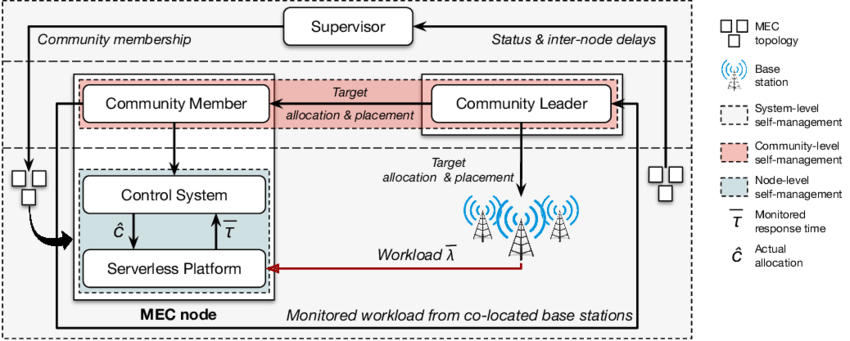
\includegraphics[width=\textwidth]{StructurePAPS.png}
    \label{fig:structure}
    \caption{PAPS general structure}
\end{figure}

\subsubsection*{System level}
Since MEC topologies can be really large and densely connected, the first step is to \textit{partition}
the network in multiple delay-aware sub-networks called \textit{communities}. Each community
is composed by a set of nodes whose propagation delay from one another is below a given 
threshold. PAPS assumes the availability of a \textit{supervisor} that has a global view of
the MEC topology and uses the SLPA \cite{SLPA} algorithm to create the communities.
\par
SLPA is an algorithm which uses label spreading techniques to decide to which community each node will belong.
It is composed of a variable number of iterations (stable solutions are obtained with 20) where nodes spread their labels 
around to their neighbors.
The main component of this  algorithm is the memory inside each SLPA node, in which it will store all the labels received.
\\
In each iteration, all the nodes will become one at a time 
\textit{listener} and will collect a label, selected from the memory, from any nearby 
node (\textit{speaker}). Once all the labels are collected, the listener selects the 
most popular node (or selects a node with any other listening rule) and adds it to its
memory.
An iteration ends when all the nodes have been listener once. \\
Since the initial idea of this 
algorithm was developed to divide social networks profiles in communities, it can create 
overlapping node which will belong to more than one community. 
In PAPS a node that is a member of multiple communities will have to balance its resources in order to address
the requests coming from different community leaders.
Each community will
elect a \textit{leader} which will be in charge of managing the community and the communication
between the nodes.

\begin{figure}[h]
    \centering
    \subfloat[SLPA Pseudocode]{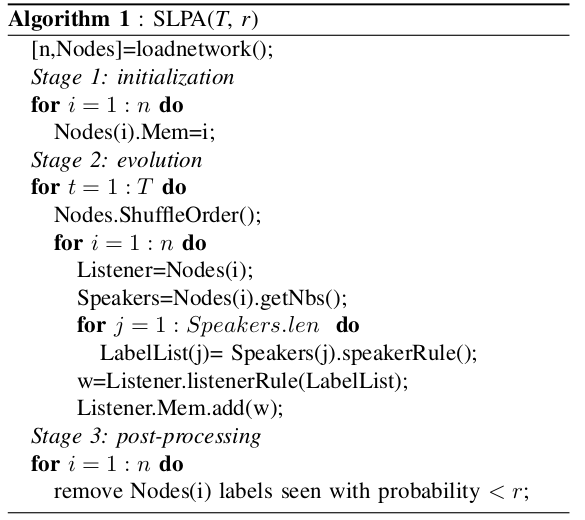
\includegraphics[width=.4\linewidth]{SLPAPseudocode.png}}%
    \label{fig:pseudocode}
    \subfloat[An example of communities division]{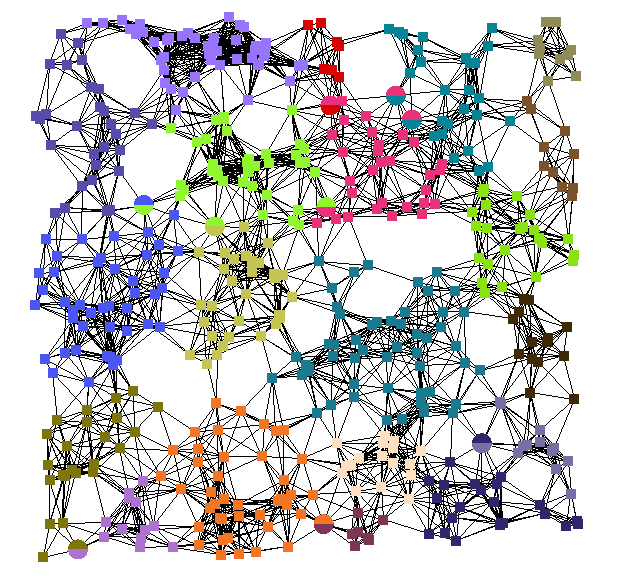
\includegraphics[width=.4\linewidth]{PPAP_communities.png}}
    \label{fig:communities}
\end{figure}

\subsubsection*{Community level}
Communities aims to minimize the likelihood of SLA violations so that the MEC nodes
can operate under feasible conditions.\\
A community leader has to supervise its community, by ensuring that every node it's still up and running.
A heart-bit signal for each node is checked inside the community.
Each community leader will manage the \textit{allocation and placement} phases by looking at 
the aggregate demand to each service and the node capacities in order to decide how to 
distribute resources among the nodes in its community. This is done solving a \textit{mixed
integer programming (MIP)} problem whose goal is to minimize the overall community delay. 
The MIP is solved periodically by the community leader which will then contact the other members
to communicate the new configuration.
Informed load balancers will use the information contained in this plan to route the workload 
coming from different base stations to the actual destination.

\subsubsection*{Node level}
The Node-Level Self-Management system aims to keep the response time for a given function fixed, 
by deploying and removing containers accordingly to the measured workload.
In order to achieve this, every node has a controller for each function that is hosting; all the controllers
run in parallel and independently.
Each controller accepts as input the number of container allocated for its function and the 
measured arrival rate, and outputs the response time. The objective is to keep the response time
at the control set point, which must be lower than the SLA.
\\
\\
Currently PAPS is a prototype that works on a simulated network in PeerSim,
in which the serverless functions are implemented as java threads. The prototype runs on a single machine and simulates
the workload by drawing from a set of probability distributions.
The goal of our project is to integrate PAPS with real world frameworks, in order to test and have a better
idea about the feasibility of this project on a real multi-node environment.
